% Compile with LuaLaTeX

\documentclass{article}

\usepackage{amsmath,geometry,graphicx,array,makecell,enumitem,bm,booktabs,multirow,pgfplots,bm,amssymb,mathtools}
\usepackage[amsmath]{ntheorem}
\usepackage[hidelinks,naturalnames]{hyperref}
\usepackage[nameinlink,noabbrev]{cleveref}
\usepackage{fancyhdr}
\usepackage{pstricks}
\usepackage{pst-electricfield}


\pagestyle{fancy}
\fancyhead[L]{\itshape\nouppercase{\leftmark}}
\fancyhead[R]{C10 Surfaces and Interfaces}


\title{Surfaces and Interfaces}
\author{Yue Wu}

\geometry{a4paper,hmargin=1.1in,vmargin=1.2in}

\setlength{\parskip}{1em}
\tolerance=1000
\emergencystretch=1em
\hyphenpenalty=1000
\exhyphenpenalty=100
\righthyphenmin=3
\addtolength\intextsep{0.2cm}

\theoremstyle{plain}\theoremheaderfont{\normalfont\itshape}\theorembodyfont{\rmfamily}\theoremseparator{.}\newtheorem*{rem}{Remark}\newtheorem*{ex}{Example}\newtheorem*{proof}{Proof}\newtheorem*{altp}{Alternative proof}

\theoremstyle{plain}\theoremheaderfont{\normalfont\bfseries}\theorembodyfont{\rmfamily}\theoremseparator{.}\newtheorem{thm}{Theorem}[section]\newtheorem{lem}[thm]{Lemma}\newtheorem{prop}[thm]{Proposition}\newtheorem*{cor}{Corollary}\newtheorem{defn}[thm]{Definition}\newtheorem{clm}[thm]{Claim}\newtheorem{clminproof}{Claim}\newtheorem*{law}{Law}\newtheorem{pos}[thm]{Postulate}

\theoremstyle{break}\theoremheaderfont{\normalfont\itshape}\theorembodyfont{\rmfamily}\theoremseparator{.\medskip}\newtheorem*{proofskip}{Proof}\newtheorem*{exs}{Examples}\newtheorem*{rems}{Remarks}

\theoremstyle{break}\theoremheaderfont{\normalfont\bfseries}\theorembodyfont{\rmfamily}\theoremseparator{.\medskip}\newtheorem{lemskip}[thm]{Lemma}\newtheorem{defnskip}[thm]{Definition}\newtheorem{propskip}[thm]{Proposition}\newtheorem{thmskip}[thm]{Theorem}

\crefname{thm}{Theorem}{Theorems}\crefname{defn}{Definition}{Definitions}\crefname{lem}{Lemma}{Lemmas}\crefname{lemskip}{Lemma}{Lemmas}\crefname{cor}{Corollary}{Corollaries} \crefname{prop}{Proposition}{Propositions}\crefname{clm}{Claim}{Claims}\crefname{pos}{Postulate}{Postulates}

\setcounter{tocdepth}{2}
\numberwithin{equation}{section}
\counterwithin{figure}{section}

\newcommand{\qed}{\hfill\ensuremath{\Box}}
\newcommand{\unit}[1]{\ \mathrm{#1}}
\newcommand{\tp}{^\mathrm{T}}
\newcommand{\dd}[2][]{\mathrm{d}^{#1} #2\,}
\renewcommand{\d}[2][]{\mathrm{d}^{#1} #2}
\newcommand{\dv}[3][]{\frac{\mathrm{d}^{#1}#2}{\mathrm{d}#3^{#1}}}
\newcommand{\pdv}[3][]{\frac{\partial^{#1} #2}{\partial #3^{#1}}}
\newcommand{\vb}[1]{\bm{\mathrm{#1}}}
\newcommand{\vu}[1]{\hat{\bm{\mathrm{#1}}}}
\newcommand{\vdot}{\,\bm{\mathrm{\cdot}}\,}
\newcommand{\abs}[1]{\left| #1 \right|}
\newcommand{\norm}[1]{\left\| #1 \right\|}
\newcommand{\grad}{\vb{\nabla}}
\renewcommand{\div}{\vb{\nabla}\cdot}
\newcommand{\curl}{\vb{\nabla}\times}
\newcommand{\laplacian}{\nabla^2}
\newcommand{\A}{\mathrm{A}}
\newcommand{\B}{\mathrm{B}}
\newcommand{\bulk}{\text{bulk}}
\newcommand{\surf}{\text{surf}}
\renewcommand{\Re}{\operatorname{Re}}
\renewcommand{\Im}{\operatorname{Im}}


\pgfplotsset{compat=1.18}
\usetikzlibrary{calc,arrows.meta,decorations.markings}

\begin{document}
    \setlength{\parindent}{0pt}
	\Huge\textsf{\textbf{Surfaces and Interfaces}}
		
	\Large\textsf{\textbf{University of Cambridge Part II Natural Sciences Tripos}}

	\noindent\makebox[\linewidth]{\rule{\textwidth}{2pt}}

	\large\textsf{\textbf{Yue Wu}}
	\begin{itemize}[topsep=0pt,leftmargin=15pt]
		\item[] \textit{Yusuf Hamied Department of Chemistry\\
		Lensfield Road,\\
		Cambridge, CB2 1EW}\\

		\textit{yw628@cam.ac.uk}
	\end{itemize}
	\thispagestyle{empty}
    \pagenumbering{roman}
	\setlength{\parindent}{15pt}

    \newpage
    \begin{center}
		\textbf{\Large{Acknowledgements}}
	\end{center}
	\large
	Nothing in these lecture notes is original. They are largely based on the notes by Prof. Stuart Clarke, Dr. David Madden and Prof. Stephen Jenkins, who lectured this course or wrote the official handout in 2025. They are nowhere near accurate representations of what was actually lectured, and in particular, all errors are almost surely mine.

	\normalsize
    \newpage
	\tableofcontents
	\newpage
    \pagenumbering{arabic}

    \section{Surfaces and Interfaces}
	In this course we are concerned with the boundary between two phases.
	\begin{defn}
		A \textit{surface} is the boundary between a condensed phase (solid or liquid) and a vapour (or vacuum) phase. An \textit{interface} is the boundary between two condensed phases.
	\end{defn}
	However, it is not uncommon to loosely call both of them ``surfaces''.

	This course can be loosely divided into three parts. The first part is mainly concerned about wet interfaces, the second part is mainly about dry, solid surfaces, and the final part is on adsorption.

	Let's first investigate some basic properties of the surfaces.

	\subsection{Surface Tension and Surface Free Energy}
	The creation of surfaces and interfaces often come with energy costs. This is known as the \textit{surface free energy} (or just \textit{surface energy}). This is easily understood if we consider a crystal structure in which there are cohesive interactions between neighbouring atoms holding materials together. A surface molecule has fewer neighbouring molecules compared with the bulk, so in order to create a surface, energy must be supplied to compensate the reduction of cohesive interactions.

	\begin{figure}[ht!]
		\centering
		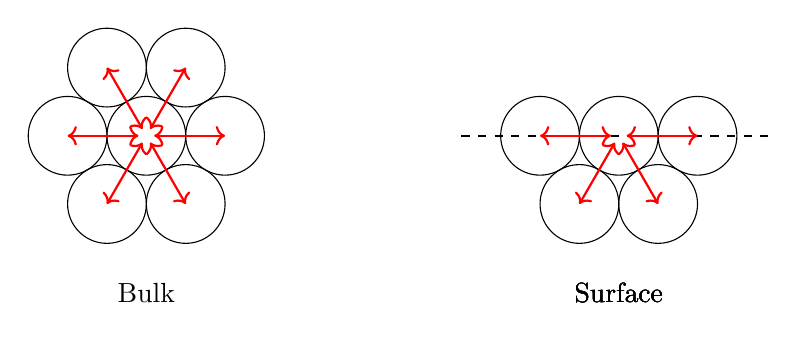
\begin{tikzpicture}
			\draw (0,0) circle (0.5);
			\foreach \i in {0,...,5}{
				\draw (\i*60:1) circle (0.5);
				\draw[<->,thick,red] (\i*60:0.1) -- (\i*60:1);
			}
			\node at (0,-2) {Bulk};

			\begin{scope}[shift={(6,0)}]
				\draw (0,0) circle (0.5);
				\draw[thick,dashed] (-2,0)--(2,0);
				\foreach \i in {3,...,6}{
					\draw (\i*60:1) circle (0.5);
					\draw[<->,thick,red] (\i*60:0.1) -- (\i*60:1);
					\node at (0,-2) {Surface};
				}
			\end{scope}
		\end{tikzpicture}
		\caption{In this simple model of 2D close-packed circular atoms, a bulk atom would form 6 favourable cohesive interactions with neighbouring atoms, while a surface atom can only form 4 such interactions.}
	\end{figure}

	Suppose the cohesive interaction is pairwise additive, and the (negative) cohesive energy between two neighbouring particles \(\A\) is \(\epsilon_{\A\A}\). The interaction with any particles further than the first neighbours are negligible. The bulk coordination number is \(z_{\A,\bulk}\) and the surface coordination number is \(z_{\A,\surf}\). Then the (positive) bulk cohesive energy per particle is
	\begin{equation}
		E_{\A,\bulk}=\frac{\Delta H_{\text{vap},\A}}{N_a}=-\frac{z_{\A,\bulk}\epsilon_{\A\A}}{2}\,,
	\end{equation}
	and so we may calculate \(\epsilon_{\A\A}\) experimentally by
	\begin{equation}
		\epsilon_{\A\A}=-\frac{2\Delta H_{\text{vap},\A}}{z_{\A,\bulk} N_A}\,,
	\end{equation}
	where \(N_A\) is the Avogadro's constant. Similarly, the cohesive energy per surface molecule is
	\begin{equation}
		E_{\A,\surf}=-\frac{z_{\A,\surf}\epsilon_{\A\A}}{2}\,.
	\end{equation}
	We assume that the nearest neighbour spacing in the surface is approximately the same as the bulk, so the nearest neighbour interaction energy \(\epsilon_{\A\A}\) is unchanging. Because \(z_{\A,\surf}<z_{\A,\bulk}\), we clearly reduce the cohesive energy by bringing a bulk particle onto the surface. This leads to an energy cost per molecule of
	\begin{equation}\label{cohesive_energy_change}
		\delta E=-(E_{\A,\surf}-E_{\A,\bulk})=-\frac{1}{2}(z_{\A,\bulk}-z_{\A,\surf})\epsilon_{\A\A}\,.
	\end{equation}

	Therefore, if we are creating a surface (e.g. cleaving a metal into two halves), we need to do some work that is proportional to the number of surface atoms formed, and hence proportional to the area \(\delta A\) of the new surface.
	\begin{equation}
		\delta w=\gamma\delta A\,.
	\end{equation}
	The proportionality constant is the \textit{surface free energy}. It has both entropic and enthalpic contributions, but for solids, the entropic change is usually negligible. By (\ref{cohesive_energy_change}), we may estimate \(\gamma\) by
	\begin{equation}
		\gamma=-\frac{1}{2}(z_{\A,\bulk}-z_{\A,\surf})\epsilon_{\A\A}N_s\,,
	\end{equation}
	where \(N_s\) is the number of molecules per surface area. Note that \(\gamma\) is positive.

	\begin{ex}
		Consider a fcc crystal, for which the bulk coordination number is 12 and the \((111)\) surface atom coordination number is 9.
		
		If we denote the close pack distance as \(a\), then the area per surface atom is \(\frac{\sqrt{3}}{2}a^2\), and so
		\begin{equation}
			N_s=\frac{2}{\sqrt{3}a^2}\,.
		\end{equation}
		Hence, the surface free energy of an fcc \((111)\) surface is
		\begin{equation}
			\gamma(111)=-\frac{3}{2}\epsilon_{\A\A}N_s=\frac{\Delta H_{\text{vap}}}{2N_A\sqrt{3}a^2}\,.
		\end{equation}
	\end{ex}

	Unlike the surface energy, the \textit{interface} energy can either be positive or negative, depending on the relative size of \(\epsilon_{\A\A}\), \(\epsilon_{\A\B}\) and \(\epsilon_{\B\B}\), where \(\A\) and \(\B\) denote the two types of particles of the two interfaces. If the interface energy is positive, i.e. the formation of interface unfavourable, then the interface will shrink to a minimum possible area. If it is negative, then the interface will tend to grow and the phases will tend to dissolve in one another. Due to the entropy contribution which we have so far ignored, dissolution may occur even if the surface energy (enthalpic) is slightly positive.

	From how we defined the surface energy \(\gamma\), it is clear that it should have dimension \(\mathrm{J}\unit{m}^{-2}\). This can also be rewritten as \(\mathrm{N}\unit{m}^{-1}\), force per unit length. This hints that the surface energy may have some alternative interpretations. Let's imagine a soap film suspended on a wire loop with one of its sides movable.

	\begin{figure}[ht!]
		\centering
		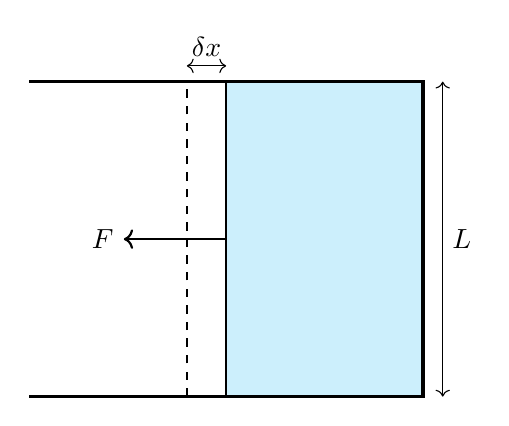
\begin{tikzpicture}
			\fill[cyan!20] (0,-2) rectangle (2.5,2);
			\draw[very thick] (-2.5,2)--(2.5,2)--(2.5,-2)--(-2.5,-2);
			\draw[thick] (0,-2)--(0,2);
			\draw[thick,dashed] (-0.5,-2)--(-0.5,2);
			\draw[thick,->] (0,0)--(-1.3,0)node[left]{\(F\)};
			\draw[<->] (-0.5,2.2)--node[above]{\(\delta x\)}(0,2.2);
			\draw[<->] (2.75,-2)--node[right]{\(L\)}(2.75,2);
		\end{tikzpicture}
		\caption{A soap film in a wire loop.}
	\end{figure}

	The soap film wants to contract in order to minimise its surface area, therefore exerting a force \(F\) on the movable side. If we pull this side with force \(F\) by a distance \(\delta x\), remembering that the film has two surfaces (up and down), the total increase in area is \(2l\delta x\), and hence the work needed to create this surface is
	\begin{equation}
		\delta w=\gamma\delta A=2\gamma l\delta x\,.
	\end{equation}
	The force exerted by the two surfaces of the film on the side of length \(l\) is therefore
	\begin{equation}
		F=\frac{\delta w}{\delta x}=2\gamma l\,,
	\end{equation}
	where each surface exerts a force
	\begin{equation}
		F=\gamma l\,.
	\end{equation}
	Hence, the \textit{surface tension}, defined as the force exerted by a surface per unit length, is exactly the surface free energy
	\begin{equation}
		\gamma=\frac{F}{l}\,.
	\end{equation}
	For liquid-liquid and liquid-vapour interfaces, the equilibrium values of \(\gamma\) is independent of the direction, so the surface tension is uniform. This is different for solid interfaces.

	The number of surface molecules is usually a very small fraction of those in the bulk. It makes an important contribution only
	\begin{enumerate}[topsep=0pt,label=(\roman*)]
		\item for a process where the bulk energy does not change;
		\item for very small particles (\(\sim\unit{nm}\)) where the surface energy becomes comparable to the bulk energies.
	\end{enumerate}

	\subsubsection{Measurement of Surface Tension}
	The most common method of measuring the surface tension is to use a \textit{Wilhelmy Plate}. Suppose the dry weight of the plate is \(W_0\), and when dipped into water, the measured weight becomes \(W\). Suppose the buoyancy force is negligible and the contact angle is \(\theta\), then the surface tension is
	\begin{equation}
		\gamma=\frac{W-W_0}{t\cos\theta}\,,
	\end{equation}
	where \(t\) is the wetted perimeter (2 width \(+\) 2 thickness).

	\begin{figure}[ht!]
		\centering
		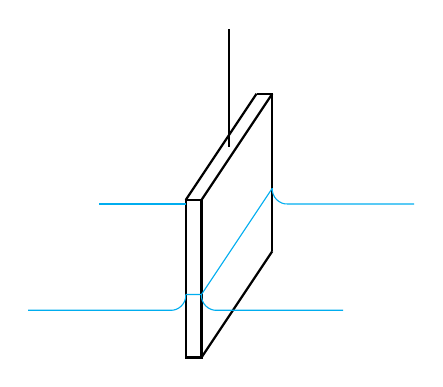
\begin{tikzpicture}[z={(0.3cm,0.45cm)}]
			\draw[thick] (0,0) rectangle (0.2,2);
			\draw[thick] (0,2,0)--(0,2,3);
			\draw[thick] (0.2,2,0)--(0.2,2,3);
			\draw[thick] (0.2,0,0)--(0.2,0,3);
			\draw[thick] (0.2,0,3)--(0.2,2,3)--(0,2,3);
			\draw[cyan] (0,0.8,0)--(0.2,0.8,0)--(0.2,0.8,3);
			\draw[cyan] (0.2,0.8,0) to[bend right=50] (0.4,0.6,0)--(2,0.6,0);
			\draw[cyan] (0.2,0.8,3) to[bend right=50] (0.4,0.6,3)--(2,0.6,3);
			\draw[cyan] (0,0.8,0) to[bend left=50] (-0.2,0.6,0)--(-2,0.6,0);
			\draw[cyan] (0,1.95)--(-2,0.6,3);
			\draw[thick] (0.1,2,1.5)--(0.1,3.5,1.5);
		\end{tikzpicture}
		\caption{A Wilhelmy plate.}
	\end{figure}

	\subsection{Contact Angle}
	One of the most common interfacial systems in everyday life is a single drop of water on a solid surface. In some cases the drop will spread and completely cover the surface, in which case we say the water completely \textit{wet} the surface. In other cases the water will form a droplet on the surface. In this case the water does not completely wets the surface.

	We characterise the wetting nature of such a solid/liquid/gas combination by the \textit{contact angle}, \(\theta\), illustrated in the figure below. It is defined to be the angle between the surface plane and the tangent to the fluid surface at the point of contact. Take care that this angle is measured inside the liquid phase.

	\begin{figure}[ht!]
		\centering
		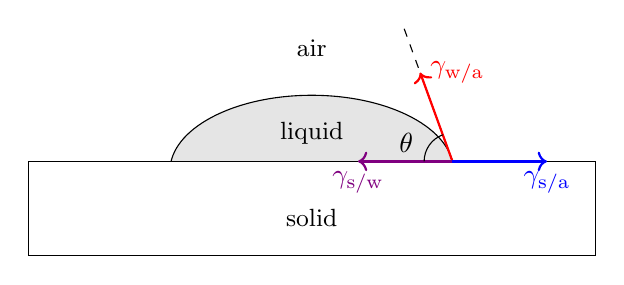
\begin{tikzpicture}[scale=1.2]
			\draw[fill=gray!20] (0,-0.1) ellipse (1.5cm and 0.8cm);
			\draw[fill=white] (-3,0) rectangle (3,-1);
			\draw[dashed] (1.49,0) --+ (110:1.5);
			\draw[thick,->,red] (1.49,0) --+ (110:1)node[right]{\(\gamma_{\text{w/a}}\)};
			\draw[thick,->,blue] (1.49,0) --+ (0:1)node[below]{\(\gamma_{\text{s/a}}\)};
			\draw[thick,->,violet] (1.49,0) --+ (180:1)node[below]{\(\gamma_{\text{s/w}}\)};
			\node at (0,0.3) {\small liquid};
			\node at (0,1.2) {\small air};
			\node at (0,-0.6) {\small solid};
			\draw (1.19,0) arc (-180:-250:0.3);
			\node at (1,0.2) {\(\theta\)};
		\end{tikzpicture}
		\caption{A liquid droplet on a solid surface. The phase labelled `air' may be another liquid phase, in which case the corresponding interfacial tensions should be used.}
	\end{figure}

	The contact angle results from the three interfacial free energies at the contact point all trying to reduce their surface area. Having identified the surface energy being the same as the surface tension (force per unit length), we can see that the horizontal components of the three surface tension forces should also balance at the point of contact, otherwise the point of contact would move and the system is not in equilibrium. This gives us the \textit{Young's equation}
	\begin{equation}\label{Youngs_equation}
		\gamma_{\text{s/a}}=\gamma_{\text{s/w}}+\gamma_{\text{w/a}}\cos\theta\,.
	\end{equation}

	The contact angle is a measure of `wettability'. If the water does not like the surface (high \(\gamma_{\text{s/w}}\)), then the drop can avoid contacts with the surface by increasing the contact angle. In the upper limit of \(\theta=180^\circ\), we say the surface is completely dry. On the other hand, if \(\gamma_{\text{s/a}}\ge\gamma_{\text{s/w}}+\gamma_{\text{w/a}}\), the formation of a liquid layer in between the solid/air surface is clearly energetically favourable, so the contact angle would be \(0^\circ\). In this case we say the surface is completely wet, or it spreads on the surface. For \(0^\circ<\theta<90^\circ\), the surface is incompletely wet and for \(90^\circ<\theta<180^\circ\), the surface is incompletely dry. A common hydrophobic material in everyday life is Teflon (PTFE) which has a contact angle with water of \(120^\circ\).

	\subsubsection{Rough Surfaces}
	The Young's equation holds for flat surfaces. When the surface is rough, an approximate equation for the contact angle actually observed is given by
	\begin{equation}
		\cos\theta_{\text{obs}}=r\cos\theta_{\text{flat}}\,,
	\end{equation}
	where \(r\) is the roughness ratio given by the ratio between the actual and projected solid surface area of a surface. It is unity for a flat surface and greater than one for any surface not completely flat. This equation is based on the assumption that the liquid penetrates into the valleys of the rough surface. Note that the direction of the change in apparent contact angle depends on value of the contact angle relative to \(90^\circ\). If the contact angle for the flat surface is bigger than \(90^\circ\), then the roughness will make the apparent contact angle even bigger, giving rise to \textit{superhydrophobic materials}. However, if the contact angle of the flat surface is less than \(90^\circ\), then roughness will decrease the apparent contact angle, leading to \textit{superhydrophilicity}.

	We can understand superhydrophobicity (superhydrophilicity) by considering the movement of the water front over a rough surface. As the water moves a short distance across the surface, the actual area of the new, unfavourable contacts is much more than the flat surface. Hence the surface appears to have a much bigger contact angle. This is the origin of the superhydrophobic nature of the lotus leaf.

	\subsection{Calculation of Free Energies of Interfaces}
	We usually have tabulated values of surface free energies (i.e. between some phase with the air), but we rarely have the interfacial free energies between any two phases of interests. It would be nice if there is some way to calculate the interfacial free energy from the surface free energies of the two individual phases.

	The basic idea would be decomposing the surface free energy into different contributions, and one then estimates these different contributions by a series of measurements using liquids with known behaviours. The overall interfacial free energy between two materials can then be calculated using some combination rules.

	\subsubsection{Owens--Wendt Method}
	The Owens--Wendt method decomposes the surface free energy into two contributions: a dispersion term and a polar term
	\begin{equation}
		\gamma=\gamma^{\text{d}}+\gamma^{\text{p}}\,.
	\end{equation}
	Some values for common solids and liquids are shown below.

	\begin{table}[ht!]
		\centering
		\begin{tabular}{cccc}
			\toprule
			Material & \(\gamma^{\text{d}}\,/\unit{mJ}\unit{m}^{-2}\) & \(\gamma^{\text{p}}\,/\unit{mJ}\unit{m}^{-2}\) & \(\gamma\,/\unit{mJ}\unit{m}^{-2}\) \\ \midrule
			\multicolumn{4}{c}{Liquids} \\ \midrule
			hexadecane & 27.8 & 0.0 & 27.8 \\
			\(\alpha\)-bromonaphthalene & 44.4 & 0.0 & 44.4 \\
			diiodomethane & 50.8 & 0.0 & 50.8 \\
			ethane diol & 29.0 & 19.0 & 48.0 \\
			formamide & 39.0 & 19.0 & 58.0 \\
			water & 21.8 & 51.0 & 72.8 \\
			mineral oil & 25.0 & 0.0 & 25.0 \\
			olive oil & 31.4 & 1.6 & 33.0 \\
			sunflower oil & 33.6 & 0.0 & 33.6 \\ \midrule 
			\multicolumn{4}{c}{Solids} \\ \midrule
			quartz & 52.0 & 44.0 & 96.0 \\
			glass & 42.0 & 34.0 & 76.0 \\
			PET & 35.0 & 4.0 & 39.0 \\
			PVC & 43.0 & 4.0 & 47.0 \\
			skin & 40.0 & 8.0 & 48.0 \\
			PE & 30.0 & 1.3 & 31.3 \\
			PP & 27.0 & 0.1 & 27.1 \\
			PTFE & 17.0 & 0.6 & 17.6 \\
			stainless steel & 33.8 & 6.2 & 40.0 \\ \bottomrule
		\end{tabular}
	\end{table}

	For two materials in contact, the interfacial free energy is given by
	\begin{equation}
		\gamma_{12}=\gamma_1+\gamma_2-2\sqrt{\gamma_1^{\text{d}}\gamma_2^{\text{d}}}-2\sqrt{\gamma_1^{\text{p}}\gamma_2^{\text{p}}}\,.
	\end{equation}
	For the particular case of a liquid drop on a solid in air, the contact angle is
	\begin{equation}
		\cos\theta=-1+\frac{2}{\gamma_{\text{l}}}\left(\sqrt{\gamma_{\text{s}}^{\text{d}}\gamma_{\text{l}}^{\text{d}}}+\sqrt{\gamma_{\text{s}}^{\text{p}}\gamma_{\text{l}}^{\text{p}}}\right)\,.
	\end{equation}
	
	For example, if one would like to measure the surface free energy of a solid, one can first measure the contact angle of a non-polar liquid (e.g. hexadecane), from which we can calculate \(\gamma_{\text{s}}^{\text{d}}\). Then we would measure the contact angle of any liquid with non-zero dispersive surface energy, from which we can obtain \(\gamma_{\text{s}}^{\text{p}}\).

	\subsubsection{Good-van Oss-Chaudhury Theory}
	It breaks the surface free energy into a dispersive and a term for acidity (\(\gamma^+\)) and basicity (\(\gamma^-\)), also known as electron acceptor and donating term
	\begin{equation}
		\gamma=\gamma^{\text{d}}+2\sqrt{\gamma^+\gamma^-}\,.
	\end{equation}
	The combination rule for the interfacial free energy is
	\begin{equation}
		\gamma_{12}=\left(\sqrt{\gamma_1^{\text{d}}}-\sqrt{\gamma_2^{\text{d}}}\right)^2+2\left(\sqrt{\gamma_1^+}-\sqrt{\gamma_2^+}\right)\left(\sqrt{\gamma_1^-}-\sqrt{\gamma_2^-}\right)\,,
	\end{equation}
	and the contact angle in air is
	\begin{equation}
		\cos\theta=-1+\frac{2}{\gamma_{\text{l}}}\left(\sqrt{\gamma_{\text{s}}^{\text{d}}\gamma_{\text{l}}^{\text{d}}}+\sqrt{\gamma_{\text{s}}^+\gamma_{\text{l}}^-}+\sqrt{\gamma_{\text{s}}^-\gamma_{\text{l}}^+}\right)\,.
	\end{equation}

	\newpage
	\section{Surface Measurement Techniques I}
	As we shall see later, it is often very difficult to study surfaces experimentally. This is because the surface material is usually only a tiny fraction of the bulk, and the surface is sometimes inaccessible when sandwiched between two phases. Ideally, we would want techniques that are \textit{surface specific}, which means that only information from the surface will be detected, and the bulk material will show no signal. In many cases the technique will only be \textit{surface sensitive} with a large contribution from the surface, but there are still some bulk contributions.

	\subsection{Vibrational Spectroscopy}
	In the same way that vibrational spectroscopy is a key way of identifying the species present in the bulk, vibrational spectroscopy at a surface is a key method to identify what is adsorbed at an interface and provides key chemical information.

	\subsubsection{Reflection Absorption Infra-Red Spectroscopy}

	The first method we introduce is the \textit{reflection absorption infra-red spectroscopy} (\textit{RAIRS}). In this method an IR beam is bounced off the surface of interest, and the absorption at each wavelength characterised in the usual way. This method \textit{per se} is neither surface specific nor surface sensitive: both the surface and the bulk materials would absorb the beam. However, we have many ways to enhance the contribution from the surface to make it more surface sensitive.
	
	For example, if we are interested in the adsorption of molecules on a solid-liquid interfaces, after a molecule is strongly adsorbed to the solid surface, the bulk fluid will be removed hence there is rather little bulk fluid material to adsorb the IR other than the molecules at the surface.
	
	Usually this experiment is performed at grazing incidence so there is a long footprint of the IR beam to enhance the surface contribution. There is also a geometric term that enhances the surface IR signal when the IR beam is at grazing incidence.

	\begin{figure}[ht!]
		\centering
		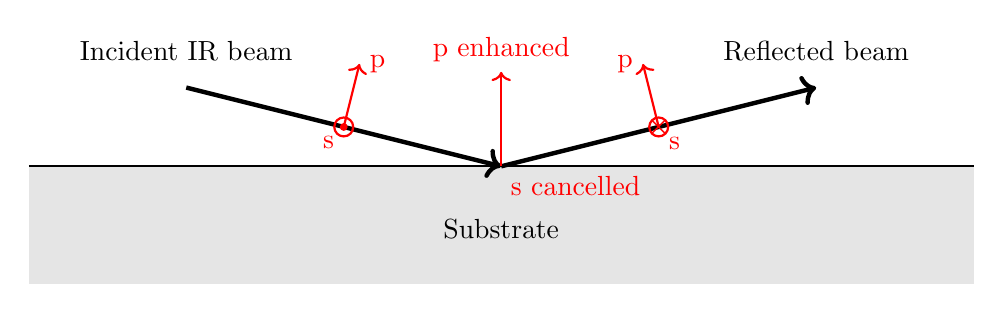
\begin{tikzpicture}
			\fill[gray!20] (-6,-1.5) rectangle (6,0);
			\node at (0,-0.8) {Substrate};
			\draw[thick] (-6,0)--(6,0);
			\draw[ultra thick,->] (-4,1)node[above=0.2cm]{Incident IR beam}--(0,0);
			\draw[ultra thick,->] (0,0)--(4,1)node[above=0.2cm]{Reflected beam};
			\draw[red,->,thick] (-2,0.5)--+(0.2,0.8)node[right]{p};
			\fill[red] (-2,0.5)node[below left]{s} circle (0.05);
			\draw[red,thick] (-2,0.5) circle (0.12);
			\draw[red,->,thick] (2,0.5)--+(-0.2,0.8)node[left]{p};
			\node[red] at (2,0.5) {\small \(\bm{\times}\)};
			\draw[red,thick] (2,0.5)node[below right]{s} circle (0.12);
			\draw[red,thick,->] (0,0)--(0,1.2)node[above]{p enhanced};
			\node[red] (0,0)[below right]{s cancelled};
		\end{tikzpicture}
		\caption{Experimental setup of RAIRS where the beam is incident at grazing angle. The s-polarised beam is cancelled on a conducting surface and the p-polarised beam is enhanced at grazing angle.}
	\end{figure}

	As we all know from A3: \textit{High Resolution Molecular Spectroscopy}, to show an IR spectrum, a molecule must have a changing dipole moment during the vibration. For RAIRS on conducting surfaces, we have a stronger selection rule known as the \textit{surface selection rule}. It states that RAIRS can only observe dipole moments oriented perpendicular to the surface. There are two primary reasons for this.
	\begin{itemize}[topsep=0pt]
		\item The electric field must be perpendicular to a conductor surface, as any tangential components of the electric field will cause free charge carriers in the conductor move to remove this tangential component.
		
		This invokes the concept of the ``image charge''. For any charge \(q\) outside the conductor, there must also be an ``image charge'' of opposite charge \(-q\) at the mirror image position, as shown in \cref{Fig:image_charge}. This is created by the movement of charge carriers in the conductor, and is necessary to keep the electric fields perpendicular at the conductor surface.

		\begin{figure}[ht!]
			\centering
			\begin{tikzpicture}
				\node at (0,0){
					\begin{pspicture*}(-5,-3.2)(5,3.2)
						\psframe*[linecolor=white](-5,-3.2)(5,3.2)
						\psElectricfield[Q={[1 -1.8 0][-1 1.8 0]}, arrowscale=1.2]
					\end{pspicture*}
				};
				
				\draw[fill=blue!10] (1.8,0) node{\(-q\)} circle (0.4);
				\draw[fill=red!10] (-1.8,0) node{\(+q\)} circle (0.4);
				\draw[very thick, dashed] (0,-3)--(0,3);
			\end{tikzpicture}
			\caption{An image charge has to be created so that the electric field is perpendicular to the conductor surface.}
			\label{Fig:image_charge}
		\end{figure}

		Therefore, for a dipole parallel to the conducting surface, there will be a image dipole in the opposite direction embedded in the surface that will cancel the source dipole (effectively forming a quadrupole). Therefore, RAIRS is unable to detect any dipole parallel to a conducting surface due to such cancellation. However, if there is a dipole perpendicular to the conducting surface, the image dipole will lie in the same direction such that the original dipole is enhanced. These effects are shown in \cref{Fig:image_dipole}.

		\begin{figure}[ht!]
			\centering
			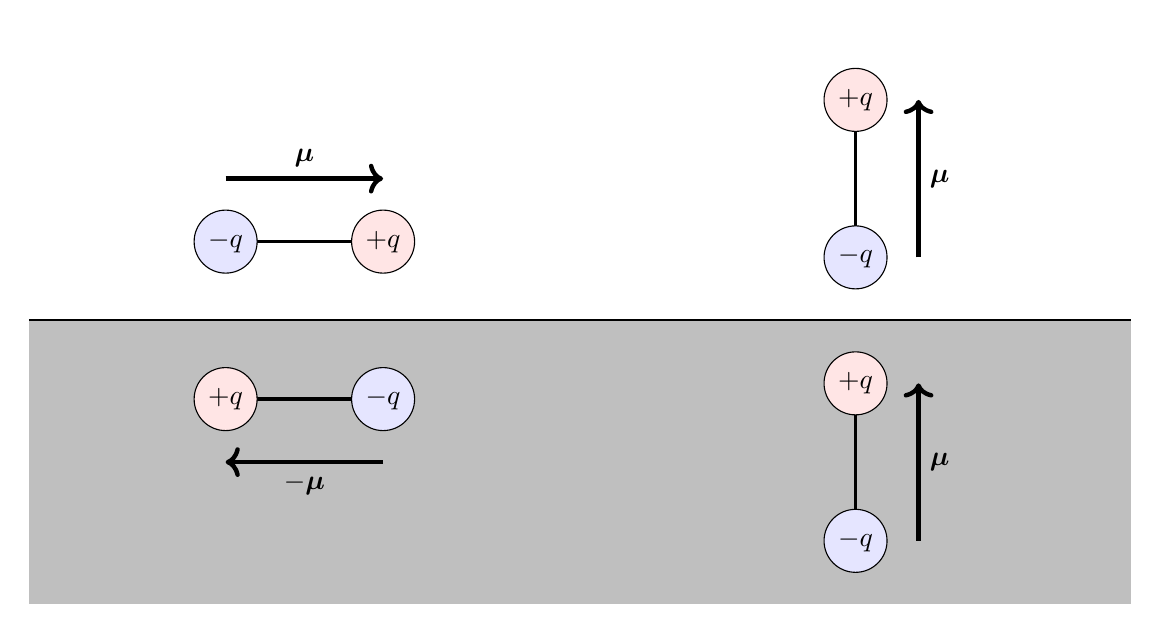
\begin{tikzpicture}
				\node at (-3.5,0){
					\begin{pspicture*}(-3,-3.6)(3,3.6)
						\psframe*[linecolor=white](-3,-3.6)(3,3.6)
						\psElectricfield[Q={[1 1 1][-1 1 -1][1 -1 -1][-1 -1 1]}, arrowscale=1.5,linewidth=0.4pt,linecolor=gray]
					\end{pspicture*}
				};

				\node at (3.5,0){
					\begin{pspicture*}(-3,-3.6)(3,3.6)
						\psframe*[linecolor=white](-3,-3.6)(3,3.6)
						\psElectricfield[Q={[1 0 2.8][-1 0 0.8][1 0 -0.8][-1 0 -2.8]}, arrowscale=1.5,linewidth=0.4pt,linecolor=gray]
					\end{pspicture*}
				};

				\fill[gray, opacity=0.5] (-7,-3.6) rectangle (7,0);
				\draw[thick] (-7,0)--(7,0);

				\coordinate (n) at (-4.5,1);
				\coordinate (p) at (-2.5,1);
				\coordinate (nim) at (-2.5,-1);
				\coordinate (pim) at (-4.5,-1);
				\draw[very thick] (n)--(p);
				\draw[fill=blue!10] (n)node{\(-q\)} circle (0.4);
				\draw[fill=red!10] (p)node{\(+q\)} circle (0.4);

				\draw[very thick] (nim)--(pim);
				\draw[fill=blue!10] (nim)node{\(-q\)} circle (0.4);
				\draw[fill=red!10] (pim)node{\(+q\)} circle (0.4);

				\draw[ultra thick, ->] (-4.5,1.8)--node[above]{\(\vb{\mu}\)}(-2.5,1.8); 
				\draw[ultra thick, ->] (-2.5,-1.8)--node[below]{\(-\vb{\mu}\)}(-4.5,-1.8); 

				\coordinate (nv) at (3.5,0.8);
				\coordinate (pv) at (3.5,2.8);
				\coordinate (nvim) at (3.5,-2.8);
				\coordinate (pvim) at (3.5,-0.8);

				\draw[very thick] (nv)--(pv);
				\draw[fill=blue!10] (nv)node{\(-q\)} circle (0.4);
				\draw[fill=red!10] (pv)node{\(+q\)} circle (0.4);

				\draw[very thick] (nvim)--(pvim);
				\draw[fill=blue!10] (nvim)node{\(-q\)} circle (0.4);
				\draw[fill=red!10] (pvim)node{\(+q\)} circle (0.4);

				\draw[ultra thick, ->] (4.3,0.8)--node[right]{\(\vb{\mu}\)}(4.3,2.8); 
				\draw[ultra thick, ->] (4.3,-2.8)--node[right]{\(\vb{\mu}\)}(4.3,-0.8); 
				
			\end{tikzpicture}
			\caption{The parallel dipoles cancel and the perpendicular dipoles enhance. The electric field lines are also plotted for reference to confirm that they are indeed perpendicular to the conductor surface as requested.}
			\label{Fig:image_dipole}
		\end{figure}

		\item The polarisation of the IR light can be decomposed into two components: a component perpendicular to the surface (p) and a component parallel to the surface (s). Light is also an oscillating electric field, so the parallel component (s-polarised light) is cancelled at the surface, while the perpendicular component (p-polarised light) is enhanced. In IR absorption, the orientation of the oscillating dipole moment of the molecule relative to the electric field vector of the incoming IR light determines the interaction strength. If the dipole oscillates parallel to the electric field, then there will be a strong absorption, while if it is perpendicular, then there will be no absorption. Since only p-polarised light survives, only oscillating dipoles perpendicular to the surface are seen.
		
		One can actually exploit the difference in behavior of s and p polarization lights observed at the surface, which is not observed as a beam passes through a bulk sample, to enhance the surface sensitivity. This gives rise to the method called PM-IRRAS (polarization modulation-infrared reflection absorption spectroscopy).
	\end{itemize}

	Low frequency modes (\(<600\unit{cm}^{-1}\)) are not generally observable in RAIRS, so hence metal-ligand bonds are not seen. Studies generally focus on the modes in adsorbed chemical groups/species, having frequencies (\(600\sim 3600\unit{cm}^{-1}\)).

	\begin{ex}
		\textit{RAIRS spectrum of MUA.}

		Below is the RAIRS spectrum of MUA (\(\mathrm{SH(CH_2)_{11}CO_2H}\)) recorded on gold, with \(85^\circ\) incidence angle, for which the \(y\)-axis is the reflectance (percentage of light reflected).
		\begin{figure}[ht!]
			\centering
			\includegraphics[width=0.6\textwidth]{RAIRS_MUA_Au.jpg}
			\caption{RAIRS spectrum of MUA on \(\mathrm{Au}\) surface.}
		\end{figure}

		As pointed earlier, the metal surface selection rule applies so no modes oriented in the plane of the surface are visible. There is a strong \(\mathrm{O-H}\) stretch at around \(3200\sim 3400\unit{cm}^{-1}\). This could be from water on the surface or residual alcohol from the self-assembly process (a type of chemistry to form molecular layers, the reaction of gold with an alkyl thiol). There are two clear \(\mathrm{C-H}\) stretches from the alkyl chain, at around \(2850\sim 2950\unit{cm}^{-1}\). There is no hydrogen bonding bands from the acid visible. The thiol \(\mathrm{S-H}\) (\(2550\sim 2600\unit{cm}^{-1}\)) is absent as there is a gold sulfur bond instead (the \(\mathrm{S-H}\) has reacted). The \(\mathrm{C=O}\) acid stretch is absent either because it is oriented in the plane of the metal or because the film is present as a carboxylate, as indicated by the symmetric and anti-symmetric carboxylate bands around 1500 cm-1. Note the reflectance value (equivalent to transmittance for a bulk IR spectrum) is very high for the RAIRS spectrum as this is a self-assembled monolayer film, one molecule thick.
	\end{ex}

	\begin{ex}
		\textit{RAIRS spectra of glycine.}

		Below is the RAIRS spectra of glycine dosed on \(\mathrm{Cu}\{311\}\) surface at \(300\unit{K}\) with increasing coverage, with a table of assignment.

		\begin{figure}[ht!]
			\centering
			\includegraphics[width=0.51\textwidth]{RAIRS_Gly_Cu.jpg}
			\qquad
			\begin{tabular}[b]{ccc} \toprule
				\multicolumn{2}{c}{On \(\mathrm{Cu}\{311\}\)} & \multirow{2}{*}{Assignment} \\
				\makecell[l]{Low \\ coverage} & \makecell[l]{High \\ coverage} & ~ \\ \midrule
				2902 & 2902 & \(\nu_{\text{as}}(\mathrm{CH_2})\) \\\midrule
				2860 & 2856 & \(\nu_{\text{s}}(\mathrm{CH_2})\) \\\midrule
				~ & 1628 & \(\nu_{\text{as}}(\mathrm{CO_2})\) \\\midrule
				1574 & 1576 & \(\delta_{\text{s}}(\mathrm{NH_2})\) \\\midrule
				~ & ~ & \(\delta_{\text{s}}(\mathrm{CH_2})\) \\\midrule
				1414 & 1416 & \(\nu_{\text{s}}(\mathrm{CO_2})\) \\\midrule
				1335 & 1335 & \multirow{2}{*}{\(\omega(\mathrm{CH_2})\)} \\
				~ & 1315 & ~ \\\midrule
				~ & 1176 & \multirow{5}{*}{\(\omega(\mathrm{NH_2})+\nu(\mathrm{CN})\)} \\
				~ & 1136 & ~ \\
				1097 & 1097 & ~ \\
				1070 & ~ & ~ \\
				1018 & 1018 & ~ \\\midrule
				960 & 960 & \(\nu_{\text{s}}(\mathrm{CC})\) \\\midrule
				947 & 947 & \(\rho_{\text{s}}(\mathrm{CH_2})\) \\ \bottomrule
			\end{tabular}
			\caption{RAIRS spectra of glycine on \(\mathrm{Cu}\{311\}\) surface at different coverages.}
		\end{figure}

		Note that at low coverages (\(<1\unit{L}\)), there is a peak at \(1414\unit{cm}^{-1}\) (carboxylate symmetric stretch) but not at \(1628\unit{cm}^{-1}\) (carboxylate antisymmetric stretch). However, the carboxylate antisymmetric stretch then develops at higher coverages (\(>1\unit{L}\)).
		
		This has been interpreted the molecule has the 3-point binding geometry on the \(\mathrm{Cu}\) surface at low coverages, with \(\mathrm{N}\) and both \(\mathrm{O}\) bonded to the surface (see \cref{Fig:three_point_binding}). The two \(\mathrm{O}\) atoms in carboxylate group are equidistant from the surface, and the transition dipole for the antisymmetric stretch therefore has no perpendicular component. The \(\mathrm{N-H}\) antisymmetric stretches are absent for the same reason.

		\begin{figure}[ht!]
			\centering
			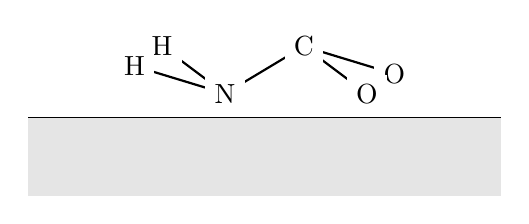
\begin{tikzpicture}
				\fill[gray!20] (-3,-1) rectangle (3,0);
				\draw (-3,0)--(3,0);
				\coordinate (H1) at (-1.65,0.65);
				\coordinate (H2) at (-1.3,0.9);
				\coordinate (N) at (-0.5,0.3);
				\coordinate (C) at (0.5,0.9);
				\coordinate (O1) at (1.3,0.3);
				\coordinate (O2) at (1.65,0.55);

				\draw[thick] (H1)--(N)--(C)--(O1);
				\draw[thick] (H2)--(N);
				\draw[thick] (C)--(O2);
				
				\node at (H2)[fill=white]{\(\mathrm{H}\)};
				\node at (H1)[fill=white]{\(\mathrm{H}\)};
				\node at (O2)[fill=white]{\(\mathrm{O}\)};
				\node at (O1)[fill=white]{\(\mathrm{O}\)};
				\node at (C)[fill=white]{\(\mathrm{C}\)};
				\node at (N)[fill=white]{\(\mathrm{N}\)};
			\end{tikzpicture}
			\caption{Coordination geometry of glycine on \(\mathrm{Cu}\{311\}\) surface at low coverages. At high coverages, some molecules will have one of their \(\mathrm{O}\) to be lifted up.}
			\label{Fig:three_point_binding}
		\end{figure}
		
		At high coverages, the surface has become much more crowded, and some glycine molecules have to lift one of their oxygens up. This becomes a two-point binding, with \(\mathrm{N}\) and only one of the \(\mathrm{O}\) bonded to the surface. The antisymmetric stretch therefore gain some perpendicular components, and the corresponding peak emerges from the spectrum.
	\end{ex}

	\subsubsection{Attenuated Total Internal Reflection Infra-Red Spectroscopy}
	The next technique is called \textit{attenuated total internal reflection infra-red spectroscopy} (\textit{ATR-IR}). It uses some specific IR-transparent crystal with a high refractive index (higher than the sample), such as diamond, and the surface of the crystal is loaded with the sample of interest. A beam of infra-red light is incident against the crystal in such a way that when it reaches the interface with the sample, the incident angle is larger than the critical angle and so the total internal reflection happens. There is an important ``side-effect'' of this total reflection called the \textit{evanescent wave}. This means that not all energies of the IR beam are being reflected, and there are some ``leakage'' of the electromagnetic wave through the interface into the sample. If the sample can absorb this electromagnetic wave (just as in the normal IR spectroscopy), then this energy is taken out of the travelling wave and we can see the corresponding peaks in the spectrum. We can record a stronger spectrum if we allow the beam to bounce off the surface for multiple times. This technique is surface sensitive because the evanescent wave decays exponentially as it passes through the sample, with a length scale of a few micrometers (the exact length depends on the wavenumber and materials \textit{etc.}).

	\begin{figure}[ht!]
		\centering
		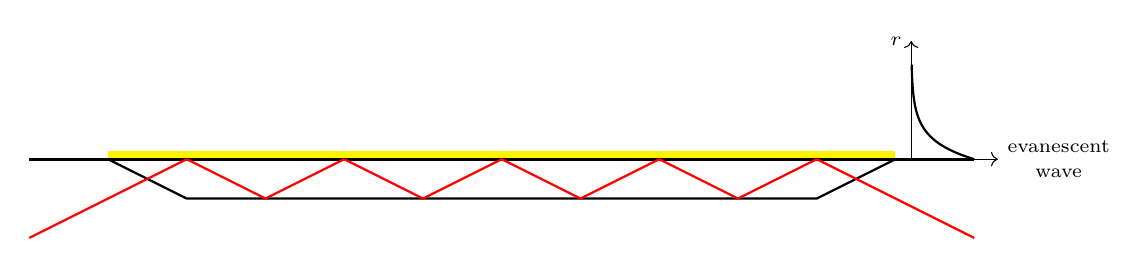
\begin{tikzpicture}
			\fill[yellow] (-5,0) rectangle (5,0.1);
			\draw[very thick] (-6,0)--(6,0);
			\draw[thick] (-5,0)--(-4,-0.5)--(4,-0.5)--(5,0);
			\draw[red,thick] (-6,-1)--(-4,0);
			\draw[red,thick] (6,-1)--(4,0);
			\foreach \i in {-3,-1,1,3}{
				\draw[red,thick](\i-1,0)--(\i,-0.5)--(\i+1,0);
			}
			\draw[->] (5.2,0)--(5.2,1.5)node[left]{\scriptsize\(r\)};
			\draw[->] (5.2,0)--(6.3,0)node[align=center,right]{\scriptsize evanescent \\[-3pt] \scriptsize wave};
			\draw[thick,domain=0:1.2, smooth, variable=\x,samples=50] plot ({5.2 + 0.8*2.8^(-4*\x)}, {\x});
		\end{tikzpicture}
		\caption{Set up of ATR-IR.}
	\end{figure}

	Since a special ATR crystal has to be used, the set up of this technique can be quite tricky. For example, if we want to investigate the adsorption of some molecules on the gold surface, we have to first deposit a very thin layer of gold on the ATR crystal, and then we can adsorb our species onto the deposited gold surface.

	\begin{ex}
		\textit{ATR-IR spectrum of MUA on diamond.}

		Below is the ATR-IR spectrum of MUA on diamond substrate.

		\begin{figure}[ht!]
			\centering
			\includegraphics[width=0.6\textwidth]{ATR_MUA.jpg}
			\caption{ATR-IR spectrum of MUA on diamond substrate.}
		\end{figure}

		The main parts of the MUA ATR spectra include the \(\mathrm{CH_2}\) stretches between \(2800\) and \(3000\unit{cm}^{-1}\). Underlying these are the acid hydrogen bonding stretches (often referred to as the old mans beard) from around \(2400\) to \(3300\unit{cm}^{-1}\). Note the weak thiol \(\mathrm{SH}\) stretch is present at close to \(2550\unit{cm}^{-1}\), indicating unreacted \(\mathrm{SH}\). Finally there is a strong \(\mathrm{C=O}\) stretch from the acid at close to \(1750\unit{cm}^{-1}\). The fingerprint region is dominated by the \(\mathrm{CH}\) bending modes.
		
		The main differences here compared to the RAIRS data of MUA on gold above reflects the different substrates and deposition methods. Here in the ATR, the MUA is deposited as a bulk sample on the diamond substrate and hence there is no reaction with the surface.
		
		Note that as the wavenumber decreases, the penetration depth of the evanescent wave increases, leading to an increasing effective thickness of the film that is probed. Hence a higher peak intensity is often observed with lower wavenumbers.
	\end{ex}

	\subsubsection{Sum Frequency Generation Spectroscopy}
	The \textit{sum frequency generation} (\textit{SFG}) spectroscopy uses two laser beams, one visible, the other in the IR region of the spectrum. This is a second order spectroscopic effect in which two photons are absorbed so that the IR absorption and Raman scattering occur simultaneously, and a photon with a frequency equal to the sum of the two input frequencies will be emitted, travelling in the direction given by the sum of the two incident wavevectors. The absorption strength is related to the hyperpolarisability of the molecule.

	\begin{figure}[ht!]
		\centering
		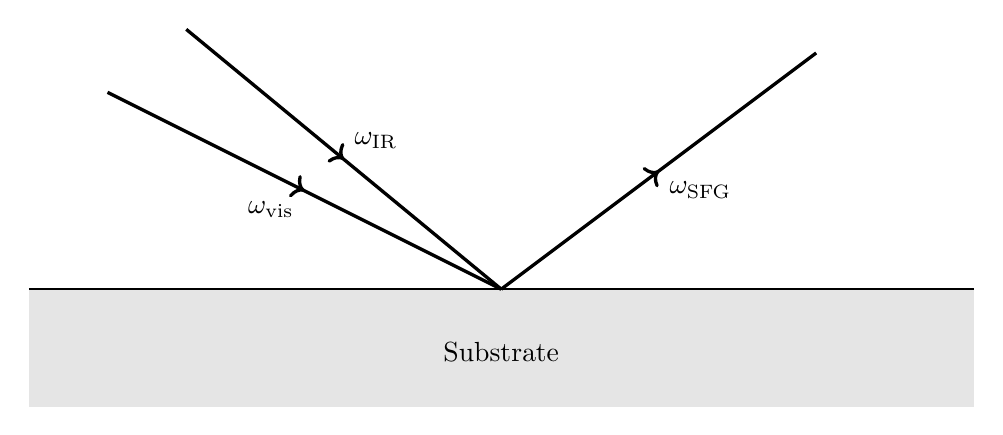
\begin{tikzpicture}[very thick,decoration={
				markings,
				mark=at position 0.5 with {\arrow{>}}}
			] 
			\fill[gray!20] (-6,-1.5) rectangle (6,0);
			\node at (0,-0.8) {Substrate};
			\draw[thick] (-6,0)--(6,0);
			\draw[postaction={decorate}] (-5,2.5)--node[below left]{\(\omega_{\text{vis}}\)}(0,0);
			\draw[postaction={decorate}] (-4,3.3)--node[above right]{\(\omega_{\text{IR}}\)}(0,0);
			\draw[postaction={decorate}] (0,0)--node[below right]{\(\omega_{\text{SFG}}\)} (4,3);
		\end{tikzpicture}
		\caption{Set up of SFG spectroscopy.}
	\end{figure}

	\begin{figure}[ht!]
		\centering
		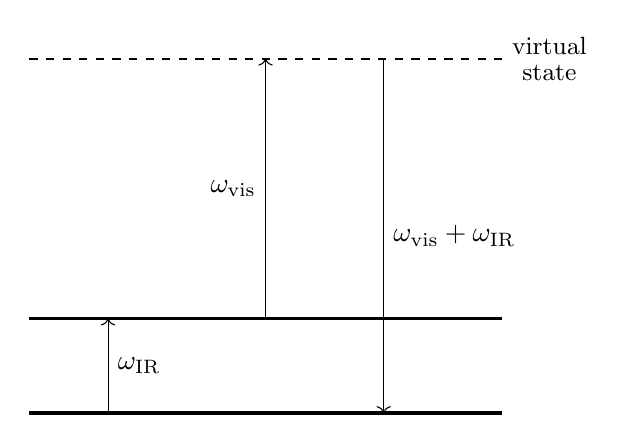
\begin{tikzpicture}
			\draw[very thick] (-3,0)--(3,0);
			\draw[thick] (-3,1.2)--(3,1.2);
			\draw[->] (-2,0)--node[right]{\(\omega_{\text{IR}}\)}(-2,1.2);
			\draw[thick,dashed] (-3,4.5)--(3,4.5)node[right, align=center]{\small virtual \\[-2.5pt]\small state};
			\draw[->] (0,1.2)--node[left]{\(\omega_{\text{vis}}\)}(0,4.5);
			\draw[->] (1.5,4.5)--node[right]{\(\omega_{\text{vis}}+\omega_{\text{IR}}\)}(1.5,0);
		\end{tikzpicture}
		\caption{In SFG spectroscopy, an IR absorption and a Raman anti-Stokes scattering happen simultaneously, and a photon of the summed frequency is emitted.}
	\end{figure}

	Note that, for this to happen, the species needs to be both IR and Raman active. The rule of mutual exclusion states that for this condition to be satisfied, the species cannot possess a centre of inversion. Bulk, centrosymmetric crystals or isotropic phases like gas or liquid can be considered to have effective centre of inversion, so they do not show such an effect. This symmetry is however broken at the surface, so only the surface contributes to the spectrum observed. This is therefore a surface specific method.

	\begin{ex}
		\textit{SFG of alkyl groups on adsorbed species.}

		The diagram shows the variation of SFG signals from alkyl groups with lower and lower coverages. This also leads to an increasing conformational disorder in the chain. Ordered chains have essentially no \(\mathrm{CH_2}\) group bands due to local inversion centres, and only \(\mathrm{CH_3}\) resonances are seen. At a slightly lower density, the \(\mathrm{CH_2}\) bands appear but due to the broken inversion symmetry. But the signals are getting weaker and weaker if we further decrease the coverage, because when the alkyl chains are free to move in space, it leads to gas/liquid like disorder, which again leads to an effective centre of inversion.

		\begin{figure}[ht!]
			\centering
			\includegraphics[width=0.7\textwidth]{SFG.jpg}
			\caption{The SFG spectra in the \(\mathrm{C-H}\) stretch region of adsorbed alkyl group.}
		\end{figure}
	\end{ex}

	\subsection{Energy Dispersive X-ray Analysis}
	It is often very important to know the elemental composition of a surface, which, in many cases, is not the same as the bulk. There are several methods to measure the surface composition of a sample. Here we will introduce a method called \textit{energy dispersive X-ray} (EDX).

	Each element has a unique electronic structure and hence a characteristic set of peaks in its X-ray spectrum from excitation between these levels. These excitations can be stimulated by electrons emitted in an electron microscope, and hence it is a standard add-on to an electron microscope. The number and energy of the X-rays emitted can be measured and analysed using an energy-dispersive spectrometer to identify the elemental composition, including the percentage of each element, of the surface.

	This technique is surface sensitive because the electrons can penetrate into the bulk material. The mean distance that the electrons penetrate is known as the \textit{electron mean free path}. Usually we probe the material a few \(\mathrm{nm}\) deep, more than just a monolayer at the surface.

	\newpage
	\section{Colloid and Curved Surfaces}
	So far, we have considered the structure and properties of planar interfaces. Now we turn our attention to small particles (e.g. grains, droplets, bubbles). The most important representatives of this class of materials in modern chemistry are nanoparticles and colloidal systems. Their large curvature introduces dramatic effects upon the properties of the system.

	\textit{Colloids} are usually considered to be tiny objects dispersed in a continuous medium: These objects are usually between \(10\unit{nm}\) and \(10\unit{\mu m}\) in size. \textit{Nanoparticles} are a subset of colloids where they range up to \(500\unit{nm}\). Note that molecules dissolved in a solution are not colloidal --- they are too small. Therefore we would describe a colloidal system as a \textit{dispersion} or a \textit{suspension} rather than a solution.

	Surface science is a key feature of nano and colloid science because when the particles get smaller, there will be a larger proportion of atoms being exposed at the surfaces.

	\subsection{Young--Laplace Equation}
	Let's consider the following case: suppose there is a spherical droplet of some phase inside another. The droplet has a radius \(r\), and the surface tension is \(\gamma\). Forming this interface has an associated (free) energy cost
	\begin{equation}
		E_{\text{surf}}=4\pi r^2\gamma\,,
	\end{equation}
	so the droplet wants to contract in order to minimise this energy cost. This leads to a slightly increased pressure in the inner phase compared with the outer phase in order to fight against this contraction. Denote the pressure of the inner phase and outer phase as \(P''\) and \(P'\), respectively, with \(P''>P'\). If the radius of the droplet change by \(\d{r}\), then the work done by the system doing so is
	\begin{equation}
		\d{W}=-P''\d{V}+P'\d{V}=-(P''-P')4\pi r^2\d{r}\,,
	\end{equation}
	while the change in the surface free energy is
	\begin{equation}
		\d{E_{\text{surf}}}=8\pi r\gamma\,\d{r}\,.
	\end{equation}
	At equilibrium, the two effects must balance, \(\d{W}+\d{E_{\text{surf}}}=0\), so
	\begin{equation}
		P''-P'=\frac{2\gamma}{r}\,.
	\end{equation}
	This is the Young--Laplace equation.

	\begin{figure}[ht!]
		\centering
		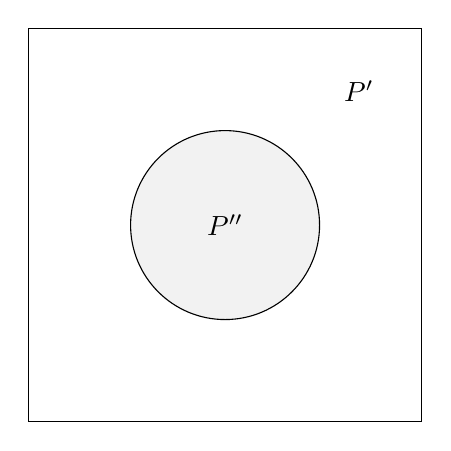
\begin{tikzpicture}
			\draw (-2.5,-2.5) rectangle (2.5,2.5);
			\draw[fill=gray!10] (0,0)node{\(P''\)} circle (1.2);
			\node at (1.7,1.7) {\(P'\)};
		\end{tikzpicture}
		\caption{The pressure inside a spherical droplet is higher than the outside phase due to surface energy.}
	\end{figure}

	\begin{ex}
		\textit{Bubbles connected by a tube.}

		Suppose we have two soap bubbles of radii \(r_1\) and \(r_2\) respectively, with \(r_1<r_2\). The pressure outside is \(P'\). Note that a bubble is a double interface (air-fluid-air), so the pressure inside is given by
		\begin{equation}
			P_i''=P'+\frac{4\gamma}{r_i}\,,
		\end{equation}
		assuming the bubble film is thin so that both the inner and outer radii are \(r_i\). Consequently, the pressure in the smaller bubble is actually higher. If we connect these two bubbles by a film, then the air will actually flow from the smaller bubble to the larger one.

		\begin{figure}[ht!]
			\centering
			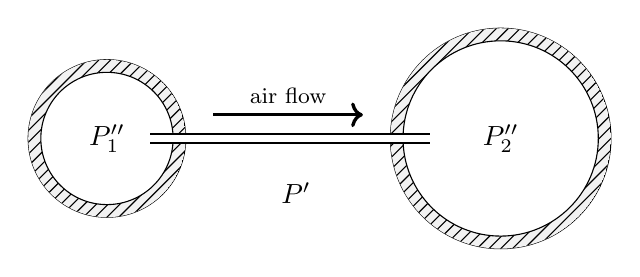
\begin{tikzpicture}
				\draw (0,0) circle (1.0);
				\begin{scope}
					\clip (0,0) circle (1.0);
					\fill[gray!10] (0,0) circle (1.0);
					\foreach \i in {-1.0,-0.85,...,3}{
						\draw (\i,1)--(-1,-\i);
					}
					\draw[fill=white](0,0) circle (0.84);
				\end{scope}
				\node at (0,0){\(P_1''\)};

				\draw (5,0) circle (1.4);
				\begin{scope}[shift={(5,0)}]
					\clip (0,0) circle (1.4);
					\fill[gray!10] (0,0) circle (1.4);
					\foreach \i in {-1.4,-1.25,...,3.4}{
						\draw (\i,1.4)--(-1.4,-\i);
					}
					\draw[fill=white](0,0) circle (1.24);
				\end{scope}
				\node at (5,0){\(P_2''\)};
				
				\fill[white] (0.55,-0.06) rectangle (4.1,0.06);
				\draw[thick] (0.55,-0.06)--(4.1,-0.06);
				\draw[thick] (0.55,0.06)--(4.1,0.06);

				\node at (2.4,-0.7) {\(P'\)};
				\draw[very thick,->] (1.35,0.3)--node[above]{\footnotesize air flow}(3.25,0.3);
			\end{tikzpicture}
			\caption{Air flows from the smaller bubble to the larger one.}
		\end{figure}
	\end{ex}

	\subsubsection{Non-Spherical Surfaces}
	Non-spherical surfaces cannot be well-described by a single radius as the radius of curvature would be different along different directions. However, it can be shown that the radii of curvature will take its maximum and minimum along two perpendicular directions on the surface (we take the radius of curvature to be negative if the surface is curved to the opposite side). These two directions are the \textit{principal axes}. Suppose the radii of curvature in these two perpendicular directions are \(r_1\) and \(r_2\), respectively. The surface divide the space into two regions, and we assign a different sign on each side of the surface. The radii of curvature with the sign included are then \(R_1\) and \(R_2\), with \(R_i=\pm r_i\), where the sign depends on the side that the centre of the inscribed circle lies. Then the \textit{local curvature} of the surface of that point is
	\begin{equation}
		J=\frac{1}{R_1}+\frac{1}{R_2}\,.
	\end{equation}

	\begin{ex}
		\textit{Local curvature.}

		\begin{figure}[ht!]
			\centering
			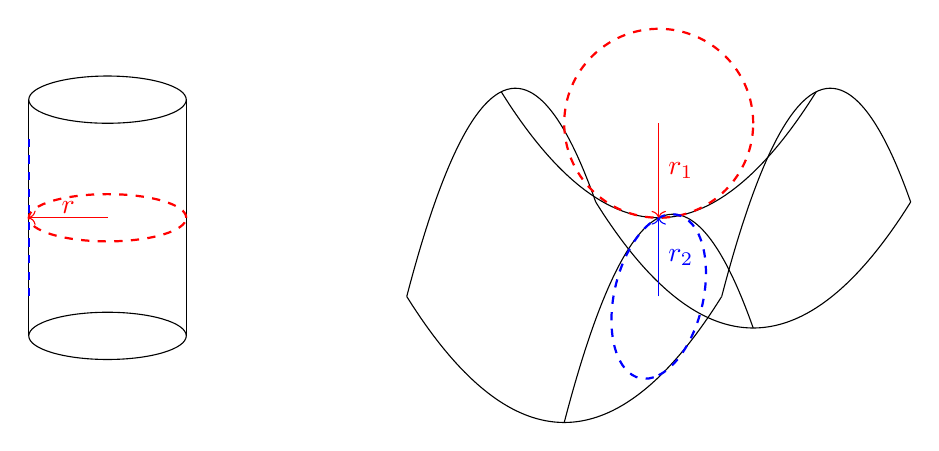
\begin{tikzpicture}
				\draw (0,0) ellipse (1 cm and 0.3cm);
				\draw (0,3) ellipse (1 cm and 0.3cm);
				\draw (-1,0)--(-1,3);
				\draw (1,0)--(1,3);
				\draw[red,thick,dashed] (0,1.5) ellipse (1cm and 0.3cm);
				\draw[red,->] (0,1.5)--node[above=-2pt]{\(r\)}(-1,1.5);
				\draw[blue,thick,dashed] (-1,0.5)--(-1,2.5);

				\begin{scope}[shift={(7,1.5)},x={(1cm,0cm)},y={(0.6cm,0.3cm)},z={(0cm,1cm)}]
					\draw[domain=-2:2, smooth, variable=\x,samples=50] plot ({\x}, {0}, {0.4*\x*\x});
					\draw[domain=-2:2, smooth, variable=\x,samples=50] plot ({\x}, {-2}, {0.4*\x*\x-2});
					\draw[domain=-2:2, smooth, variable=\x,samples=50] plot ({\x}, {2}, {0.4*\x*\x-2});
					\draw[domain=-2:2, smooth, variable=\y,samples=50] plot ({0}, {\y}, {-0.5*\y*\y});
					\draw[domain=-2:2, smooth, variable=\y,samples=50] plot ({-2}, {\y}, {-0.5*\y*\y+1.6});
					\draw[domain=-2:2, smooth, variable=\y,samples=50] plot ({2}, {\y}, {-0.5*\y*\y+1.6});
					\begin{scope}[shift={(0,0,1.2)}]
						\draw[red,thick,dashed,rotate around x=90] (0,0,0) circle (1.2);
					\end{scope}
					\begin{scope}[shift={(0,0,-1)}]
						\draw[blue,thick,dashed,rotate around y=90] (0,0,0) circle (1);
					\end{scope}
					\draw[->,red] (0,0,1.2)--node[right]{\(r_1\)}(0,0,0);
					\draw[->,blue] (0,0,-1)--node[right]{\(r_2\)}(0,0,0);
				\end{scope}
			\end{tikzpicture}
		\end{figure}

		The cylinder of radius \(r\) has local curvature
		\begin{equation}
			J=\frac{1}{r}+\frac{1}{\infty}=\frac{1}{r}\,.
		\end{equation}
		The saddle has local curvature
		\begin{equation}
			J=\frac{1}{r_1}-\frac{1}{r_2}\,.
		\end{equation}
	\end{ex}

	One can show that for a non-spherical surface, the pressure difference is given by
	\begin{equation}
		\Delta P=P_+-P_-=J\gamma\,,
	\end{equation}
	where \(P_+\) is the pressure on the side we assigned the positive sign, and \(P_-\) the pressure in the minus sign region. The pressure will be higher on the more convex side, i.e. if \(J\) is positive, then the pressure will be higher on the positive side and \textit{vice versa}. For a spherical surface, \(J=2/r\) and this reduce to the Young--Laplace equation.

	\begin{ex}
		\textit{Water between two surfaces.}

		If we spill some water on a table, put a cup on it and lift the cup by a little, the water surface will look like the figure below:
		\begin{figure}[ht!]
			\centering
			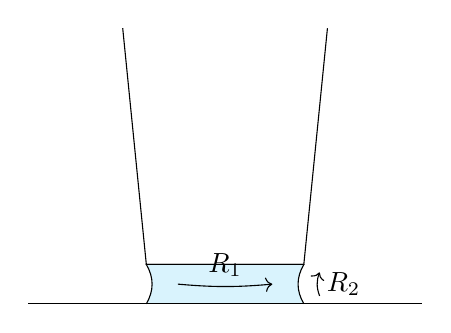
\begin{tikzpicture}
				\draw (-1.3,3.5)--(-1,0.5)--(1,0.5)--(1.3,3.5);
				\draw[fill=cyan!15] (-1,0)to[bend right](-1,0.5)--(1,0.5)to[bend right](1,0);
				\draw (-2.5,0)--(2.5,0);
				\draw[->] (-0.6,0.25) to[bend right=5] node[above]{\(R_1\)} (0.6,0.25);
				\draw[->] (1.2,0.1) to [bend left=20] node[right]{\(R_2\)} (1.2,0.4);
			\end{tikzpicture}
		\end{figure}

		We have \(\abs{R_1}\gg \abs{R_2}\), so \(1/R_2\) dominates in the curvature. The pressure in the water is lower than the pressure in the atmosphere.
	\end{ex}

	\subsubsection{Capillary Rise}
	One of the most important consequences of the Young--Laplace equation is that of capillary rise where a liquid like water will rise up (or sometimes drop down) inside a thin capillary.

	The key point is that due to the interfacial energy, the liquid must make some contact angle \(\theta\) with the capillary wall as given by Young's equation (\ref{Youngs_equation}). This makes the liquid surface curved inside the capillary, and hence there must be a pressure difference between the water and the atmosphere. This pressure difference can only be achieved if the water level in the capillary rises/drops by some amount.

	\begin{figure}[ht!]
		\centering
		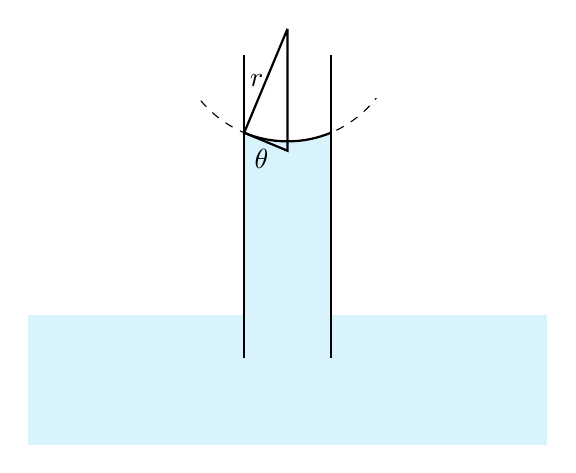
\begin{tikzpicture}[scale=1.1]
			\fill[cyan!15] (-3,0.5) rectangle (3,2);
			\fill[cyan!15] (-0.5,0.5) rectangle (0.5,4.4);
			\begin{scope}
				\clip (-3,1) rectangle (3,4.5);
				\draw[dashed, fill=white] (0,5.3) circle (1.3);
				\clip (-0.5,0.5) rectangle (0.5,5);
				\draw[thick] (0,5.3) circle (1.3);
			\end{scope}
			\draw[thick] (-0.5,1.5)--(-0.5,5);
			\draw[thick] (0.5,1.5)--(0.5,5);
			\draw[thick] (0,5.3)--node[left=-0.1cm]{\(r\)}(-0.5,4.1)--++(0.5,-0.20833)--(0,5.3);
			\node at (-0.3,3.8) {\(\theta\)};
			
		\end{tikzpicture}
	\end{figure}

	Suppose the cylindrical capillary has radius \(a\) and the contact angle between the water and the capillary wall is \(\theta\). Let's suppose the water-air interface is spherical, then the radius of curvature of this spherical interface is
	\begin{equation}
		r=\frac{a}{\cos\theta}
	\end{equation}
	Suppose the height of capillary rise is \(h\), and the atmospheric pressure above the bulk water surface is \(p_0\). Then at the capillary water-air interface, the air pressure is
	\begin{equation}
		p_{\text{air}} = p_0 - \rho_{\text{air}}gh\,,
	\end{equation}
	and the water pressure is
	\begin{equation}
		p_{\text{water}} = p_0 - \rho_{\text{water}}gh\,.
	\end{equation}
	Since the air-water interface is curved towards the water phase, the pressure in the air must be slightly higher than in the water. By the Young--Laplace equation, we must have
	\begin{equation}
		p_{\text{air}}-p_{\text{water}}=\frac{2\gamma}{r}\,,
	\end{equation}
	and so
	\begin{equation}
		hg(\rho_{\text{water}}-\rho_{\text{air}})=\frac{2\gamma\cos\theta}{a}\,.
	\end{equation}
	Since \(\rho_{\text{water}}\gg \rho_{\text{air}}\), we may ignore the air density and write
	\begin{equation}
		h=\frac{2\gamma\cos\theta}{ag\rho_{\text{water}}}\,.
	\end{equation}

	\section{Surfactants}

	\section{Surface Measurement Techniques II}



	

	

	

\end{document}